\chapter{Valence bond states}

	\section{Parent Hamiltonian}

		The usual procedure in approaching a problem is by taking its Hamiltonian, then do some perturbation theory to find the ground state of the system. The procedure of the parent Hamiltonian is to take a state $\ket \psi$ that one wants to be a ground state, from which a parent Hamiltonian will be inferred. The procedure to recover this Hamiltonian is to consider a set of operators $\{Q_\Gamma\}$ such that
		\be Q_\Gamma \ket \psi = 0 \ \forall \Gamma \ee
		which would lead to the wanted Hamiltonian
		\be \mc H = \sum_\Gamma Q_\Gamma \ee
		If one associates to $Q_\Gamma$ eigenvectors $\ket{\psi_i^\Gamma}$ forming a complete basis with eigenvalues $\lambda_i^\Gamma \geq 0$ -- which is a correct assumption since $Q_\Gamma$ are projectors -- then
		\be \begin{split} \ev{\mc H}{\phi} &= \sum_\Gamma \ev{Q_\Gamma}{\phi} \\ &= \sum_\Gamma \sum_i \mel{\phi}{Q_\Gamma}{\psi_i^\Gamma}\braket{\psi_i^\Gamma}{\phi} \\ &= \sum_\Gamma \sum_i \lambda_i^\Gamma \abs{\braket{\psi_i^\Gamma}{\phi}}^2 \geq 0 \end{split} \ee
		This means that $\ket \psi$ is a ground state but not if it is unique.

		The parent Hamiltonian may differ from the physical model, but serves to bring a light to the relations between interactions and the ground state correlations. This concept has to be tied with the variational principle since the ground state wavefunction is not analytically known for most Heisenberg models.

	\section{Valence bond}

		A valence bond state is a variational wavefunction for the antiferromagnetic Heisenberg model. This is a singlet state $|\psi_i^j\rangle$ which connects two spin-$\frac{1}{2}$ particles between sites $i$ and $j$ and thus minimizes the Heisenberg coupling. A valence bond configuration, or a dimer covering, is a tensor product of valence bond states. Examples of valence bond configurations are given in \autoref{fig:VBS1} and \autoref{fig:VBS2}. Hence, \autoref{fig:VBS1} shows a $1$D configuration out of $2$ possible, and \autoref{fig:VBS2} a $2$D one out of many. A configuration has $\vb* S_\text{tot}^2 = S_\text{tot} (S_\text{tot} +1) =0$. Also, there is in general a non-zero overlap between possible configurations. 
		
		\begin{figure}[h!]
            \centering
            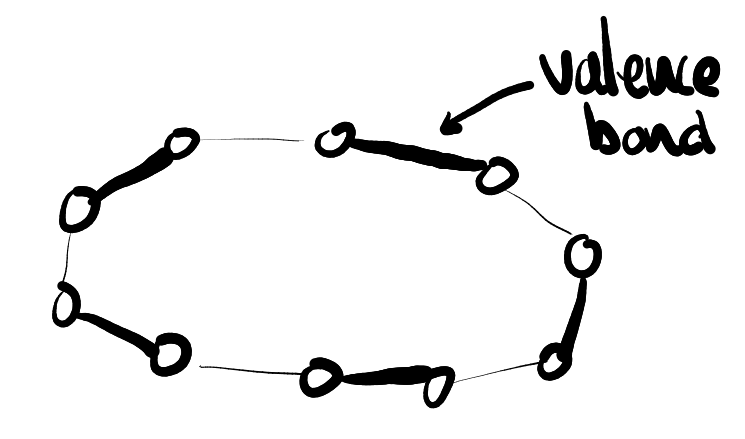
\includegraphics[scale=0.2]{graphs/VBS1.png}
            \caption{Example of valence bond configuration in $1$D.}
            \label{fig:VBS1}
        \end{figure}

		A general valence bond state is written as
		\be \ket{\{c_\alpha\}, S} = \sum_\alpha c_\alpha \ket \alpha \label{eq:vbs} \ee
		where $c_\alpha$ are variational parameters and $\alpha$ valence bond configuration, written as
		\be \ket \alpha = \prod_{(ij) \in \Lambda_\alpha} [a^\dagger_i b^\dagger_j - b^\dagger_i a^\dagger_j ]\ket 0 \ee
		with $a_i,b_i$ Schwinger bosons on site $i$ and $\Lambda_\alpha$ a particular configuration of bonds $(ij)$ on the lattice. Note that $S$ here can take any value, but one will always be able to decompose the configurations so that one can take $S=\frac{1}{2}$ in the end.

        \begin{figure}[h!]
            \centering
            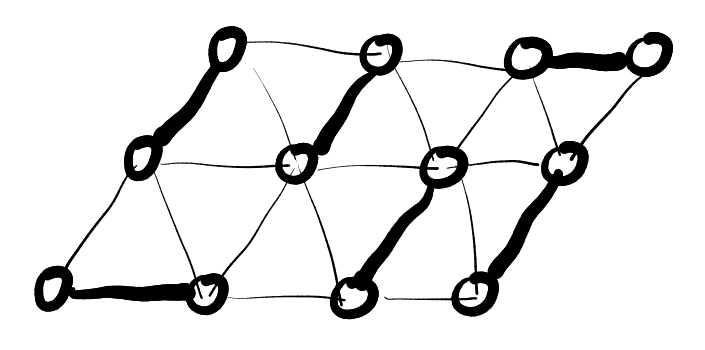
\includegraphics[scale=0.2]{graphs/VBS2.png}
            \caption{Example of valence bond configuration in $2$D.}
            \label{fig:VBS2}
        \end{figure}

		The sum in \eqref{eq:vbs} in certain cases in the large lattice limit, is made over a finite number of configurations. These cases where there are many configuration in \eqref{eq:vbs} are denoted as resonating valence bond sates.

	\section{The Majumdar-Ghosh Hamiltonian}

		Consider a $L$ unit cells $1$D chain of spin-$\frac{1}{2}$ alternate pairs of sites just as in \autoref{fig:VBS1}. They are in a singlet state with boundary $\vb* S_{L+1} = \vb* S_{1}$
		\be \ket{d_\pm} = \bigotimes_{i=1}^{L/2} \frac{1}{\sqrt 2} \left[\ket \uparrow _{2i} \ket \downarrow _{2i\pm 1} - \ket \downarrow _{2i} \ket \uparrow _{2i \pm 1}\right] \label{eq:mgdpm} \ee
		which are the only two possible configurations. The goal is to kill these states under the action of a parent Hamiltonian. To do so, find the projector of the subspace $J=\frac{3}{2}$ so that
		\be \mc P_\frac{3}{2}(i-1, i, i+1) \ket{d_\pm} =0 \ee
		where one considers $\vb* J = \vb* S_{i-1} + \vb* S_i + \vb* S_{i+1}$ and thus here $J=\frac{1}{2}, \frac{3}{2}$. Since the total spin must vanish on the $z$-sector, the only possibility is to have $J=\frac{1}{2}$. The eigenvalues of $\vb* J^2=J(J+1)$ and the projectors are presented more intuitively in \autoref{tab:Jproj}.
		\begin{table}[h!]
			\centering
			\begin{tabular}{cccc}
				& $J(J+1)$ & $\mc P_\frac{1}{2}$ & $\mc P_\frac{3}{2}$ \\ \hline
				$J=\frac{1}{2}$ & $\frac{3}{4}$ & 1 & 0 \\
				$J=\frac{3}{2}$ & $\frac{15}{4}$ & 0 & 1
			\end{tabular}
			\caption{Intuitive representation of the $J$ subspaces and their projectors.}
			\label{tab:Jproj}
		\end{table}
		Hence, one can think to take
		\be \mc P_\frac{3}{2} \propto \vb* J^2 - \frac{3}{4} \ee
		and noting that $\frac{15}{4}-\frac{3}{4} = 3$, one can write
		\be \mc P_\frac{3}{2} = \frac{1}{3} \left[ \vb* J^2 - \frac{3}{4}\right] \ee
		Therefore, substitute the expression for $\vb* J$ and expand to find
		\be \mc P_\frac{3}{2} = \frac{1}{2} + \frac{2}{3} \left[\vb* S_{i-1} \cdot \vb* S_i + \vb* S_{i-1} \cdot \vb* S_{i+1} + \vb* S_i \cdot \vb* S_{i+1} \right] \ee
		enabling to find the Majumdar-Ghosh Hamiltonian
		\be \begin{split} \mc H_\text{MG} &= \sum_{i=1}^L \mc P_\frac{3}{2}(i-1, i, i+1) \\ &= \frac{L}{2} + \frac{4}{3} \sum_{i=1}^L \left[ \vb* S_i \cdot \vb* S_{i+1} + \frac{1}{2}\vb* S_i \cdot \vb* S_{i+2}  \right] \end{split} \ee
		which by construction gives
		\be \mc H_\text{MG} \ket{d_\pm} = 0 \ee

		Now take the state
		\be \ket{\phi_\pm} = \frac{1}{\sqrt 2} \left[\ket{d_+} \pm \ket{d_-}\right] \ee
		which is correctly normalized only for $N\to \infty$. To show this, first introduce the loop covering. This is presented on \autoref{fig:loopcovering}, where one loop is shown. 
		\begin{figure}[h!]
            \centering
            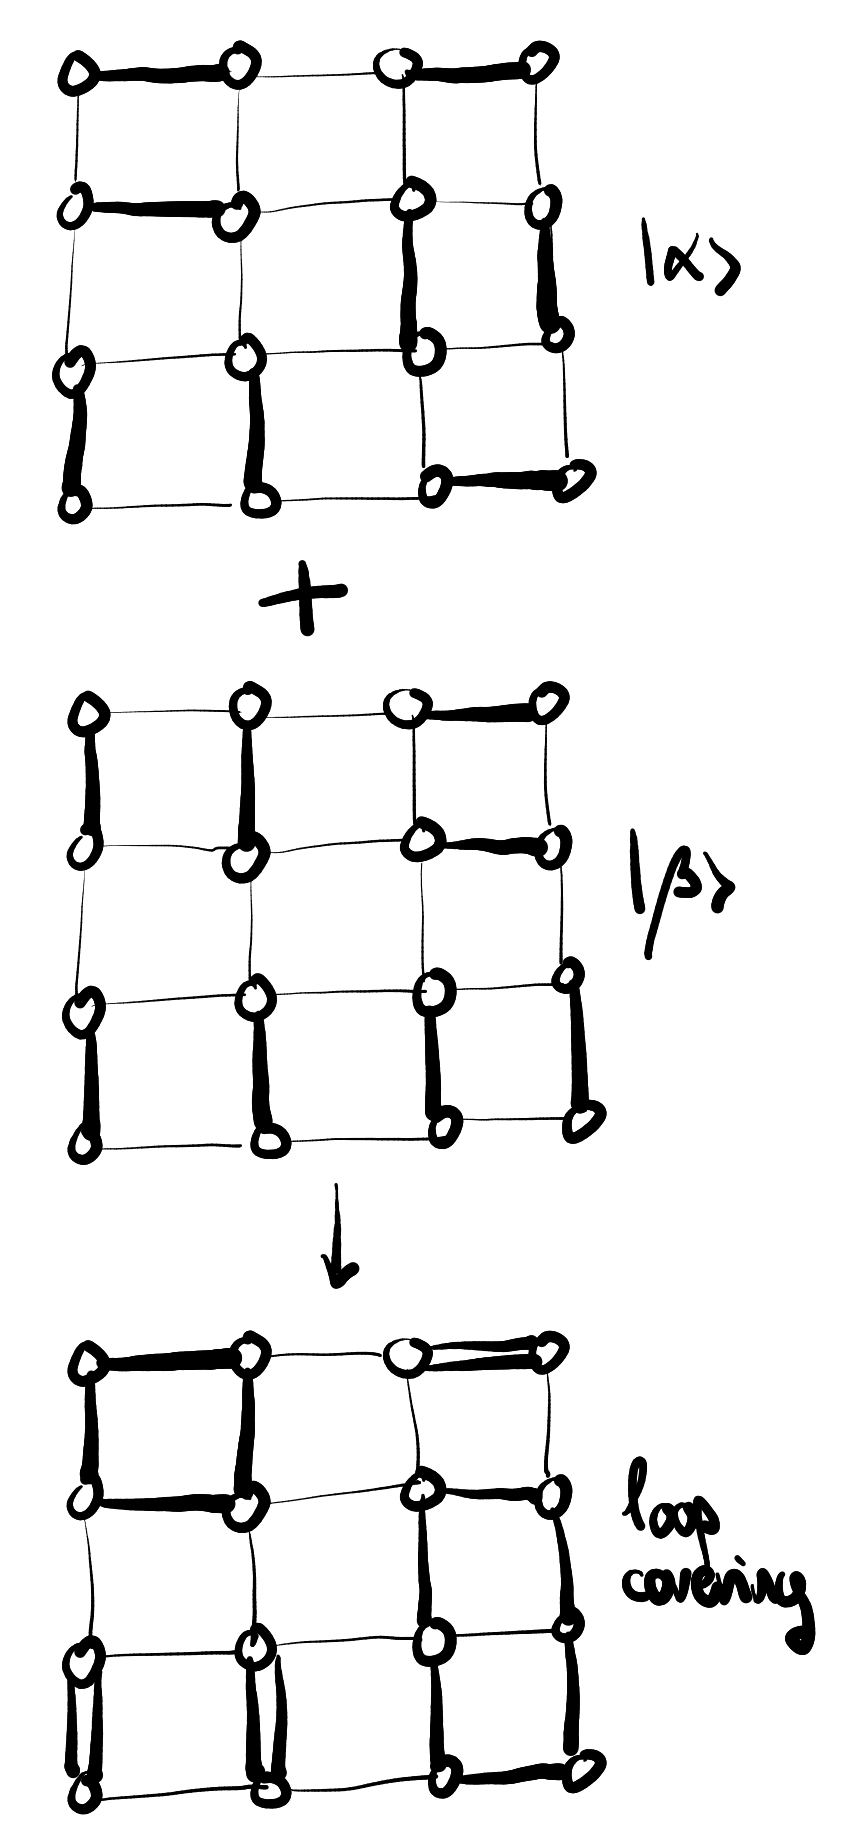
\includegraphics[scale=0.2]{graphs/loopcovering.png}
            \caption{Example of a loop covering by the overlap of two valence bond configurations on a $2$D square spin-$\frac{1}{2}$ lattice.}
            \label{fig:loopcovering}
        \end{figure}
		In general, a loop $\Gamma$ is set to have a length $2L(\Gamma)$ which is an even number of links. For a loop of length $2L(\Gamma)$, only Néel states contribute. There are two of them since flipping spin at each site also give the same loop. Each state has a weight $2^{-L(\Gamma)}$ from the singlet normalization. Hence, the overlap between states $\ket \alpha$ and $\ket \beta$ is
		\be \braket{\alpha}{\beta} = \prod_\Gamma 2 \cdot 2^{-L(\Gamma)} = 2^{\sum_\Gamma 1} 2^{-\frac{1}{2}\sum_\Gamma 2L(\Gamma)} \ee
		Now, by seeing that $N = \sum_\Gamma 2L(\Gamma)$ and writing the number of loops as $p(\ket \alpha,\ket \beta)$, one gets
		\be \braket{\alpha}{\beta} = 2^{p(\ket \alpha,\ket \beta)-\frac{N}{2}} \xrightarrow{N \to \infty} 0 \ee
		For the case of Majumdar-Ghosh states, ones finds $p(\ket{d_+}, \ket{d_-}) = 1$ and thus
		\be \braket{d_+}{d_-} = 2^{1-\frac{N}{2}} \xrightarrow{N \to \infty} 0 \ee
		Now seek for the expectation values of the spin correlations and find in the thermodynamic limit $N\to \infty$
		\be \ev{\vb* S_i \cdot \vb* S_j}{\phi_\pm} = \frac{1}{2} \left[2 \cdot\frac{3}{4} \delta_{i,j} - \frac{3}{4} \delta_{\abs{i-j},1} \right] \ee
		This can be found as follows. The $\frac{1}{2}$ in front comes from the normalization of the $\ket{\phi_\pm}$. For $i=j$, one has $\vb* S^2 = S(S+1) = \frac{3}{4}$ and the factor $2$ comes from the $2$ states $\ket{d_\pm}$ appearing in the definition of $\ket{\phi_\pm}$. For ${\abs{i-j},1}$, only one of $\ket{d_\pm}$ contributes to gives $-\frac{3}{4}$, which can be easily computed using the definition \eqref{eq:mgdpm} and the fact that
		\be \vb* S_i \cdot \vb* S_j = S_i^x S_j^x + S_i^y S_j^y + S_i^z S_j^z \ee
		with the operators acting like
		\be S^z \ket \sigma = \sigma \ket \sigma, \quad S^x \ket \sigma = \abs{\sigma} \ket{-\sigma}, \quad S^y \ket \sigma = i\sigma \ket{-\sigma} \ee
		For instance, consider only the $z$-component
		\be \begin{split} S_i^z S_j^z \ket d_+ &= \cdots \otimes \frac{1}{\sqrt 2} \left[-\frac{1}{2} \ket \uparrow _{i-1} \ket \downarrow _{i} - \frac{1}{2} \ket \downarrow _{i-1} \ket \uparrow _{i}\right] \otimes \cdots  \\ &\otimes \frac{1}{\sqrt 2} \left[-\frac{1}{2} \ket \uparrow _{j-1} \ket \downarrow _{j} - \frac{1}{2} \ket \downarrow _{j-1} \ket \uparrow _{j}\right] \otimes \cdots \end{split} \ee
		Therefore, taking $\bra{d_+}$ one finds what expected depending one the value of $i$ and $j$. Hence it is easy to see that there is no contribution when $\abs{i-j} \geq 2$.

		Overall, this is manifest of a short-range correlations, characteristic of spin liquids. This is sometimes called spin-Peierls system.

	\section{AKLT model}

		To goal is to construct a spin-$1$ wavefunction which creates spin-$\frac 1 2$ singlets on all bounds of a chain, and is the ground state of a Hamiltonian looking like the spin-$1$ Heisenberg model. The chain can be decomposed into singlet pairs as in \autoref{fig:spin1decomp}, where one can go from the singlet chain to the spin-$1$ one by applying the symmetrization operator on two neighboring ends of valence bonds, which gives state of spin $S=1$.
		\begin{figure}[h!]
            \centering
            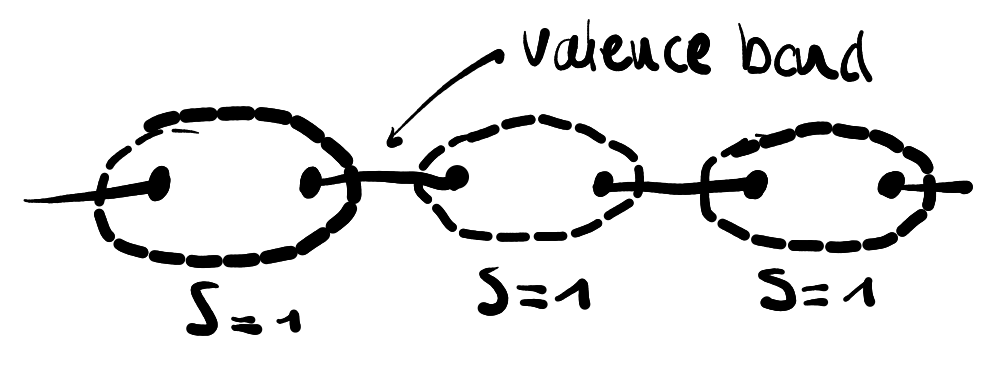
\includegraphics[scale=0.2]{graphs/spin1decomp.png}
            \caption{Example of a decomposition of a spin-$1$ lattice into a product of valence bonds.}
            \label{fig:spin1decomp}
        \end{figure}
        But start by working in the Schwinger-bosons representation
		\be S^+ = a^\dagger b, \quad S^- = b^\dagger a , \quad S^z = \frac{1}{2} \left [a^\dagger a - b^\dagger b \right] \ee
		with each boson satisfying the SU$(2)$ commutation relations, that is
		\be [ S^+, S^-] = 2 S^z, \quad [ S^\pm, S^z] = \pm  S^\pm \ee
		which can be easily checked. Also, imposing the constraint
		\be 2S = a^\dagger a + b^\dagger b \ee
		one can arrive at finding 
		\be \vb* S^2 = S(S+1) \ee
		Moreover, it can be shown that the state consisting of two spins-$\frac{1}{2}$ at $i$ and $j$
		\be \ket \phi = \frac 1{\sqrt 2} \left[a^\dagger_i b^\dagger_j - b^\dagger_i a^\dagger_j \right] \ket 0 \ee
		is the singlet, since it is correctly normalized, that 
		\be S^-_\text{tot} \ket \phi = (S^-_i + S^-_j) \ket \phi = 0 \ee
		and that
		\be S^z_\text{tot} \ket \phi = (S^z_i + S^z_j) \ket \phi = 0 \ee
		which can be rapidly recovered by noting that there is always $1$ $a$ and $1$ $b$, and that $S^z_\text{tot}$ is counting the number of $a$ minus the number of $b$ at both sites. Hence introduce
		\be \ket{\psi_\text{VBS}} = 2^{-\frac N 2} \prod_i \left[a^\dagger_i b^\dagger_{i+1} - b^\dagger_i a^\dagger_{i+1}\right] \ket 0 \ee
		which corresponds to one spin-$1$ per site. Indeed, the wavefunction has either a factor $a^\dagger_i a^\dagger_i$, $a^\dagger_i b^\dagger_i$ or $b^\dagger_i b^\dagger_i$, thus is an eigenstate of $a^\dagger_i a_i + b^\dagger_i b_i$ with eigenvalue $2$.

		Now one look for the parent Hamiltonian of which $\ket{\psi_\text{VBS}}$ is the ground state. Start by noticing that for a pair of spin-$1$
		\be S\otimes S = 1 \otimes 1 = 0 \oplus 1 \oplus 2 \ee
		that are the subspaces of $J$, and that the wavefunction contains singlets, thus spin-$2$ is impossible. Now take again the bond spin
		\be \vb* J_{i,i+1} = \vb* S_i + \vb* S_{i+1} \ee
		Recalling the scheme of \autoref{tab:Jproj}, one can find easily
		\be \mc P_2 = \frac{1}{24} \vb* J^2 (\vb* J^2-2) \ee
		since one must construct the Hamiltonian with $\mc P_2$ such that
		\be \mc P_2(i,i+1) \ket{\psi_\text{VBS}} = 0 \ee
		Hence, noting that in this case
		\be \vb* J_{i,i+1}^2 = 4 + 2 \vb* S_i \cdot \vb* S_{i+1} \ee
		the parent AKLT Hamiltonian is found as
		\be \begin{split} \mc H^\text{AKLT} &= \sum_{i=1}^N \mc P_2(i,i+1) \\ &= \frac N 3 + \frac 1 2 \sum_{i=1}^N \left[\vb* S_i \cdot \vb* S_{i+1} + \frac 1 3 \left(\vb* S_i \cdot \vb* S_{i+1}\right)^2 \right] \end{split} \ee
		where the constant term can often be omitted and the factor in front of the sum too. Note that the first term is the Heisenberg Hamiltonian and the second is a biquadratic interaction that can somehow be seen as a perturbation.\\

		For the more general case with spin $S$, taking $M=\frac{2S}{z}$ and the $1$D lattice, the valence bond solid is 
		\be \ket{\psi_\text{VBS}} = \prod_{\ev{ij}} \left[a^\dagger_i b^\dagger_j - b^\dagger_i a^\dagger_j\right]^M \ket 0 \label{eq:VBSgen} \ee
		The last paragraphs are obtained considering a correct normalization and $S=M=1$. One can see that for $m=0,1,\dotsc,\vb* S_i \cdot \vb* S_j$
		\be \left(\vb* S_i \cdot \vb* S_j\right)^m = \sum_{J=0}^{2S} \left[\frac 1 2 J(J+1) - S(S+1)\right]^m \mc P_J(i,j) \ee
		which can be inverted to find
		\be \mc P_J(i,j) = \prod_{k=0,\ k\neq J}^{2S}\frac{2\vb* S_i \cdot \vb* S_j + 2S(S+1) - k(k+1)}{J(J+1)+k(k+1)} \ee
		As before, projecting on the subspace
		\be J_{ij} > J_\text{max} = 2S-M \ee
		gives zero, so that the projector one seeks for are those. Indeed, $J^z_\text{max} = 2S-M$ is the maximal eigenvalue on $\ket{\psi_\text{VBS}}$ by counting the maximal number of $a^\dagger$ minus $b^\dagger$ in it. Since $\ket{\psi_\text{VBS}}$ is a singlet due to th product of singlets, it is rotationally invariant and thus if $J>J^z_\text{max}$, a global rotation would lead to a possible $J^z = J$ which is impossible. Thus $J^z_\text{max} = J_\text{max}$. This implies that the general parent Hamiltonian is 
		\be \mc H^\text{AKLT} = \sum_{\ev{ij}} \sum_{J=2S-M+1}^{2S} K_J \mc P_J(i,j) \qq{with} K_J \geq 0 \ee

	\section{Spin correlations}

		To calculate the spin correlations of the valence bond state \eqref{eq:VBSgen}, introduce the spin coherent states, created by applying the SU$(2)$ rotation operator to the maximally polarized state
		\be \begin{split} \ket{\hat \Omega} &= \mc R(\chi,\vartheta,\phi) \ket{S,S} \\ &= e^{iS^z \phi} e^{iS^y \vartheta} e^{iS^x \chi} \ket{S,S} \end{split} \ee
		where $\hat \Omega = (\cos\phi\sin\vartheta, \sin\phi\sin\vartheta,\cos\vartheta)$ is the unit vector is spherical coordinates. Thus $\chi$ is a gauge freedom. Schwinger bosons transform as
		\be \begin{split} \pmqty{a^\dagger \\ b^\dagger}'& = \mc R \pmqty{a^\dagger \\ b^\dagger} \mc R^{-1} \\ &= \pmqty{u e^{i\chi /2} & v e^{i\chi /2} \\ -v^* e^{-i\chi /2} & u^* e^{-i\chi /2}} \pmqty{a^\dagger \\ b^\dagger} \end{split} \ee
		with
		\be u = \cos \frac{\vartheta}{2} e^{i\phi/2} \qq{and} v = \sin \frac{\vartheta}{2} e^{-i\phi/2} \ee
		found by expanding the exponential and making use of the fact that bosons here are eigenoperators of the spin ones. Then the coherent states
		\be \begin{split} \ket{\hat \Omega} &= e^{iS\chi} \frac{(a^{\dagger\prime})^{2S}}{\sqrt{(2S)!}} \ket 0 \\ &= e^{iS\chi} \frac{(ua^\dagger +vb^\dagger)^{2S}}{\sqrt{(2S)!}} \ket 0 \\ &= e^{iS\chi} \sqrt{(2S)!} \sum_m \frac{u^{S+m} v^{S-m}}{\sqrt{(S+m)!(S-m)!}} \ket{S,m} \end{split} \ee
		where in general
		\be \ket{S,m} = \frac{(a^\dagger)^{S+m}}{\sqrt{(S+m)!}} \frac{(b^\dagger)^{S-m}}{\sqrt{(S-m)!}} \ket 0 \ee
		This allows to express the correlations as a classical statistical mechanics average. First
		\be \begin{split} \braket{\hat \Omega}{\psi_\text{VBS}} &= \sqrt{(2S)!} \prod_{\ev{ij}} (u_i v_j - v_i u_j)^M \\ &= \sqrt{(2S)!} \prod_{\ev{ij}} \left(\frac{1 - \hat \Omega_i \cdot \hat \Omega_j}{2} \right)^\frac{M}{2} \end{split} \ee
		Therefore, the spin correlations are
		\be \begin{split} \ev{\vb* S_i \cdot \vb* S_j}{\psi_\text{VBS}} &= \frac{(S+1 - \delta_{ij})(S+1)}{Z} \\ &\cdot \int\prod_i \dd\hat \Omega_i \ \abs{\braket{\hat \Omega}{\psi_\text{VBS}}}^2 \hat \Omega_i \cdot \hat \Omega_j  \end{split} \ee
		with the partition function
		\be Z = \int\prod_i \dd\hat \Omega_i \ \abs{\braket{\hat \Omega}{\psi_\text{VBS}}}^2 \ee
		In $1$D, it is possible to compute
		\be \ev{\vb* S_0 \cdot \vb* S_n}{\psi_\text{VBS}} = \begin{cases} (-1)^n (S+1)^2 e^{-\xi(S)\abs{n}} & n \neq 0 \\ S(S+1) & n=0 \end{cases} \ee
		with 
		\be \xi(S) = \ln\left(1 + \frac 2 S \right) \ee
		This means that there is no long-range order. Thus, due to short-range order, the valence bonds states in $1$D and $2$D describe quantum spin liquids, by Mermin-Wagner theorem. In $3$D, for $M$ large enough, it can be expected that the classical Hamiltonian produces long-range antiferromagnetic order, even giving rotationally invariant states.





